% Design document for the AirPLAi CV trial project.
% Build: make design   (pdflatex twice, for the table of contents)
\documentclass[10pt,a4paper]{article}

\usepackage[T1]{fontenc}
\usepackage[utf8]{inputenc}
\usepackage{charter}
\usepackage{microtype}
\usepackage[margin=18mm,top=16mm,bottom=18mm]{geometry}
\usepackage{booktabs}
\usepackage{tabularx}
\usepackage{xltabular}
\usepackage{array}
\usepackage[dvipsnames]{xcolor}
\usepackage{enumitem}
\usepackage{titlesec}
\usepackage[hang,flushmargin]{footmisc}
\makeatletter\renewcommand{\@makefntext}[1]{\raggedright\noindent\@makefnmark\,#1}\makeatother
\usepackage[font=small,labelfont=bf,skip=6pt]{caption}
\usepackage{float}
\usepackage{tikz}
\usetikzlibrary{positioning,arrows.meta,fit,backgrounds,calc}
\usepackage[colorlinks=true,linkcolor=Sepia,urlcolor=Sepia,citecolor=Sepia]{hyperref}

\definecolor{slate}{RGB}{48,56,68}
\definecolor{accent}{RGB}{198,102,36}
\definecolor{mute}{RGB}{120,128,138}

\titleformat{\section}{\large\bfseries\color{slate}}{\thesection}{0.7em}{}
\titleformat{\subsection}{\normalsize\bfseries\color{slate}}{\thesubsection}{0.6em}{}
\titlespacing*{\section}{0pt}{10pt}{4pt}
\titlespacing*{\subsection}{0pt}{7pt}{2pt}

\setlist[itemize]{leftmargin=1.2em,itemsep=2pt,topsep=3pt}
\setlength{\parskip}{2pt}
\renewcommand{\arraystretch}{1.05}
\setlength{\LTpre}{6pt}\setlength{\LTpost}{6pt}

\newcolumntype{L}[1]{>{\raggedright\arraybackslash}p{#1}}
\newcommand{\changed}[1]{%
  \par\smallskip\noindent
  {\color{accent!88!black}\small\textbf{$\triangleright$ Changed in the build.} \textit{#1}}\par\smallskip}

\title{\vspace{-16mm}\bfseries\color{slate}Dodgeball Throw-Attempt Detection\\[1mm]
       \large\mdseries Design document}
\author{Gary Ferguson}
\date{\vspace{-2mm}27 August 2026}

\begin{document}
\maketitle
\thispagestyle{empty}

\noindent
\begin{minipage}{\textwidth}
\small\color{slate}
\rule{\textwidth}{0.4pt}\\[3pt]
\textbf{What this is.} The design for a system that turns broadcast dodgeball footage
into an attributed timeline of throw attempts and one derived metric, team throw
efficiency. It covers the pipeline, the signals, the components, the data and labels,
the evaluation, the compute budget and where we expect it to break.

Decisions the build overturned are marked \textcolor{accent!88!black}{$\triangleright$}
in place; the measurement and reasoning behind each is in the report.\\[2pt]
\rule{\textwidth}{0.4pt}
\end{minipage}

\vspace{1mm}
{\small\setcounter{tocdepth}{2}\tableofcontents}
\clearpage

%=====================================================================
\section{The event}

\subsection{Why this sport, this event}

Dodgeball, because it is a less orthodox choice. As far as I can find there is no published
vision work on it, one hobbyist post on possession\footnote{A.\ Hu, `Leveraging
AI Video Frame Recognition to Quantify Ball Possession', \emph{Medium}, December 2025,
$<$\url{https://medium.com/@arthurwang0815/leveraging-ai-image-recognition-to-quantify-ball-possession-e6493d8428e1}$>$,
accessed 27 August 2026.} and a 2015 sensor-based
paper,\footnote{T.\ Nojima, N.\ Phuong,
T.\ Kai, T.\ Sato and H.\ Koike, `Augmented dodgeball', in \emph{Proceedings of the 6th
Augmented Human International Conference} (AH~'15), Singapore, 2015, pp.\ 137--140.} so there is no established approach to copy and the design has to come from
the sport and the footage. Within it, the candidates below were scored against the brief
(hard, fine-grained, temporal, attributable, with a derived metric) and against a ten-hour
budget.

{\footnotesize
\begin{xltabular}{\textwidth}{L{34mm} L{26mm} X l}
\toprule
\textbf{Sport / event} & \textbf{Temporal} & \textbf{Why it was or was not chosen} & \textbf{Verdict}\\
\midrule
Dodgeball, elimination / re-entry & Weak, a rule consequence & Crisp boundaries and trivial attribution, but it reads as ``person crosses a line'' & rejected\\
\textbf{Dodgeball, throw attempt} & \textbf{Strong} & The event does not complete at release, it stays open until the ball resolves, and feints are wind-ups that never release. The ball is only needed near the thrower, so no global ball tracking & \textbf{chosen}\\
BJJ, positional change & Strong & Entangled-body pose is unsolved at this budget and labelling needs expertise & rejected\\
Ice hockey, zone entry & Strong & Named in the brief as an example, and puck possession would dominate the budget & rejected\\
Ultimate, turnover & Strong & Viable, but less structured than the throw cascade & fallback\\
\bottomrule
\end{xltabular}}

The throw attempt was chosen for its structured negatives: a pass is identical to a throw
up to the last stage, and a feint is identical up to the second.

\subsection{The event as a cascade}

Every labelled thing starts as a \emph{candidate}, a throwing motion, and resolves down a
tree. Each level is a separate decision with its own failure mode, so ground truth is
labelled at every level and the evaluation reports every level separately
(\S\ref{sec:eval}) rather than one blended F1.

\begin{figure}[H]
\centering
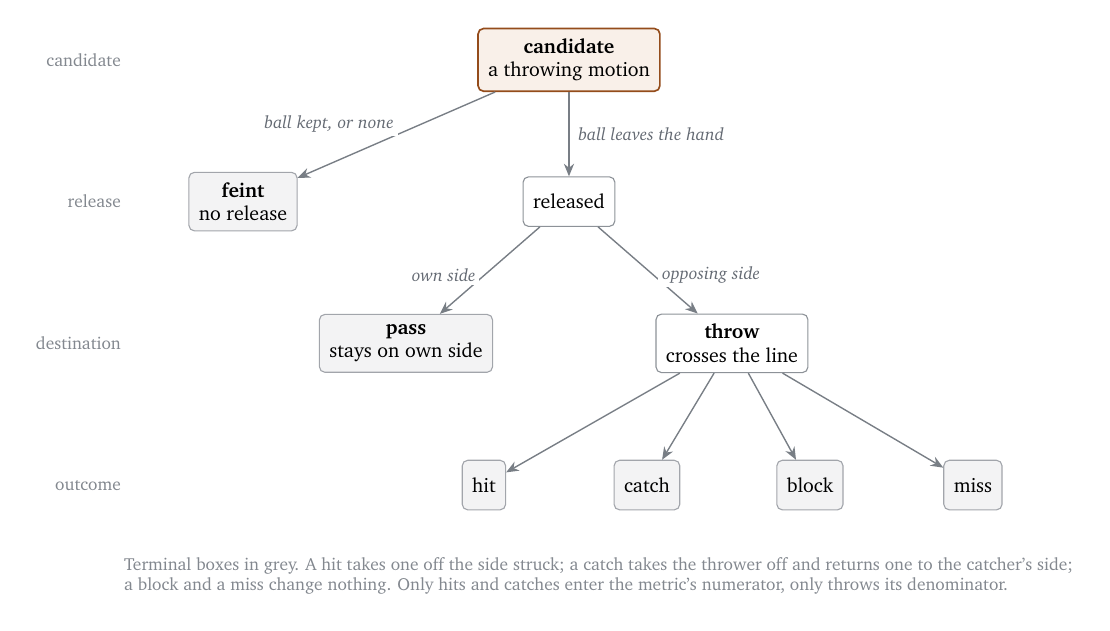
\begin{tikzpicture}[
  scale=0.9, every node/.style={transform shape},
  font=\small,
  lvl/.style={font=\scriptsize, text=slate!60, anchor=east},
  node/.style={draw=slate!55, fill=white, rounded corners=2pt, inner sep=4pt,
               minimum height=7mm, align=center, font=\footnotesize},
  cand/.style={node, draw=accent!75!black, fill=accent!10, line width=0.6pt},
  term/.style={node, draw=slate!45, fill=slate!6},
  q/.style={font=\scriptsize\itshape, text=slate!75, fill=white, inner sep=1.5pt},
  ar/.style={-{Stealth[length=1.6mm,width=1.3mm]}, draw=slate!65, line width=0.5pt},
]
\node[cand] (c) at (0,0) {\textbf{candidate}\\a throwing motion};

\node[term] (fake) at (-4.6,-2.0) {\textbf{feint}\\no release};
\node[node] (rel)  at (0,-2.0)  {released};

\node[term] (pass) at (-2.3,-4.0) {\textbf{pass}\\stays on own side};
\node[node] (thr)  at (2.3,-4.0)  {\textbf{throw}\\crosses the line};

\node[term] (hit)   at (-1.2,-6.0) {hit};
\node[term] (catch) at (1.1,-6.0)  {catch};
\node[term] (block) at (3.4,-6.0)  {block};
\node[term] (miss)  at (5.7,-6.0)  {miss};

\draw[ar] (c) -- (fake) node[q, pos=0.5, above left=-1pt] {ball kept, or none};
\draw[ar] (c) -- (rel)  node[q, pos=0.5, right=2pt] {ball leaves the hand};
\draw[ar] (rel) -- (pass) node[q, pos=0.55, left=2pt] {own side};
\draw[ar] (rel) -- (thr)  node[q, pos=0.55, right=2pt] {opposing side};
\draw[ar] (thr) -- (hit);
\draw[ar] (thr) -- (catch);
\draw[ar] (thr) -- (block);
\draw[ar] (thr) -- (miss);

\node[lvl] at (-6.2,0)    {candidate};
\node[lvl] at (-6.2,-2.0) {release};
\node[lvl] at (-6.2,-4.0) {destination};
\node[lvl] at (-6.2,-6.0) {outcome};

\node[font=\scriptsize, text=slate!60, align=left, anchor=north west] at (-6.4,-6.9)
  {Terminal boxes in grey. A hit takes one off the side struck; a catch takes the thrower off
   and returns one to the catcher's side;\\ a block and a miss change nothing. Only hits and
   catches enter the metric's numerator, only throws its denominator.};
\end{tikzpicture}
\caption{The event cascade. Four decisions in order, each with its own failure mode and its
own score.}
\label{fig:cascade}
\end{figure}

{\footnotesize
\begin{xltabular}{\textwidth}{L{22mm} L{46mm} X}
\toprule
\textbf{Level} & \textbf{Decision} & \textbf{Where it fails}\\
\midrule
Candidate & Is there a throwing motion at all? & Recall ceiling. Whatever is missed here is gone from every level below\\
Release & Did the ball leave the hand? & Occlusion at the release moment: nothing to see, not merely hard to see\\
Destination & Own side (pass) or opposing side (throw)? & Shallow releases near the centre line, lobbed passes\\
Outcome & What happened to the ball? & Graze versus dodge, catch versus drop. This is where annotators will disagree\\
\bottomrule
\end{xltabular}}

\subsection{The event definition}

The rules recognise nothing before release: a throw ``must leave a player's hand'' and the
ball is live ``once the player is no longer in contact with the ball''.\footnote{World
Dodgeball Federation, \emph{WDBF Dodgeball Rules 2024} (2024), rule 15.2,
$<$\url{https://worlddodgeballfederation.com/wdbf-content/uploads/2024/03/WDBF-Dodgeball-Rules-2024.pdf}$>$,
accessed 27 August 2026. Quoted by rule number in \texttt{docs/reference/wdbf-rules.md}.} A feint is a
coaching term, not a rule term, so what counts as one is ours to fix.

{\footnotesize
\begin{xltabular}{\textwidth}{l X}
\toprule
\textbf{Field} & \textbf{Rule}\\
\midrule
\texttt{kind} & \texttt{fake} (no release), \texttt{pass} (released, ball stays on the thrower's own side), \texttt{throw} (released, ball crosses to the opposing side). Mutually exclusive by construction\\
\texttt{start} & First frame of the wind-up: the throwing arm moves behind the shoulder line\\
\texttt{release} & First frame the ball is no longer in contact with the hand\\
\texttt{end} & The first contact that settles the ball: an opponent, a catch, a block, the floor or the far boundary\\
\texttt{actor} & Thrower, as team (required) plus player identity where the track is stable\\
\texttt{outcome} & \texttt{hit}, \texttt{catch}, \texttt{block}, \texttt{miss}, or \texttt{unresolved} (occluded or off-frame)\\
\texttt{target} & The player the ball reached, for hit / catch / block. Required, because a catch eliminates the \emph{thrower} while a hit eliminates the \emph{target}\\
\texttt{confidence} & Reported separately for (a) that a throw occurred, (b) attribution, (c) outcome\\
\bottomrule
\end{xltabular}}

\changed{Not built. Every decision is a threshold on a named quantity and that quantity is
written to the timeline (wind-up score, ball mass at the wrist, departure distance, how long
the count step held), so a confidence would be a mapping from those margins; it was not done
in the budget. Report \S2.}

Two things follow from the rules. A candidate needs no ball: an empty-handed wind-up is
still a move meant to draw the opponent, and the same motion to a stage that looks for
motions. Classification is by destination, not intent: an errant pass that crosses and
connects is a throw with a hit, since a live ball eliminates whoever it reaches. The ruleset
agrees (``passing throws and plays are not deemed invalid throws, if the ball does not cross
into the opponent team's fair territory'')\footnote{WDBF, \emph{Rules}, 16.2.} and it is
the only workable rule, because destination is observable and intent is not. A release whose
destination was never seen carries no \texttt{kind} at all and is reported separately.

\subsection{Game state as a free consistency check}

Only a throw resolving changes the on-court count: a hit takes one off the side struck, a
catch takes the thrower off and returns one to the catcher's side, a miss and a block change
nothing. Folding the timeline forward gives the count at every frame, and it has to stay
legal. On labels, a violation (seven a side, an eliminated player throwing) locates a bad
label without a second annotator. On predictions, the same fold flags impossible sequences as
false positives.

\subsection{The derived metric}

\textbf{Team throw efficiency} $=$ eliminations $\div$ throw attempts, per team per set,
split by solo versus coordinated attacks (two or more same-team releases within 300\,ms). It
is dodgeball's shooting percentage, and the split asks whether attacking together converts
more often or just spends more balls.

Its error is the cascade's. Passes and feints sit outside the denominator, so every pass
misread as a throw understates efficiency and every feint read as a throw dilutes it. The
numerator depends on outcome accuracy. The pass term is the awkward one: a pass causes no
elimination and so leaves no trace in the game-state fold, so direction is the only evidence
there is.

%=====================================================================
\section{Pipeline}
\label{sec:pipeline}

Two halves. The first sets up the context every later decision needs (where the court is,
who is on it, when the set is live) and runs once per clip. The second is the event cascade
itself, one decision per level of the tree in \S1.2.

\subsection{Setting up the context}

\textbf{Court.} Basic HSV methods pull the lines out of a median background frame and we
fit a homography to those. That gives us metres, but the thing it is mostly for is deciding
who is in play: anyone whose feet are not on the court is not a player.

\textbf{Pose.} YOLO11x-pose over every frame, once, written to disk. Both the pipeline and
the labelling tool read the same run, so ``no skeleton here'' means the same thing to both.

\textbf{Set start and end.} We detect the start of each set by looking for the balls lined
up on the centre line and a whistle while they are there, confirmed by both teams breaking
for the balls. The end is the last elimination. Throws outside a set do not count and the
metric is per set.

\textbf{Players.} Players get a team from their kit colour and an identity from ByteTrack,
with a jersey number read off the best crops where the budget allows. This is what lets us
say which side a throw came from and keep a count of who is still on court.

\subsection{The event cascade}

\textbf{Candidates.} Wrist speed, to find when something happens at all. The rest of the
cascade works out what that something was.

\textbf{Release.} HSV extraction again, this time to check for a ball in the thrower's
hands. If the ball is still there afterwards, or was never there, it was a feint.
If we can see the ball leaving, it is a throw.

\textbf{Destination.} A ball that stays on the thrower's own side is a pass; the court
homography says which side it went to.

\textbf{Outcome.} For throws at the opposing team we want hit, miss, catch or block. A ball
that flies uninterrupted to the floor or the boundary is a miss. Hit, catch and block need
other signals on top of the ball's short trajectory: does a player leave the court after it (hit), does a player rejoin
(catch), does the ball make contact and nothing changes (block). The on-court count is the
check on all of it, since only a throw resolving can move it.

\changed{The outcome is read from the count, not the ball. At 25\,fps and twenty pixels the
frame where the ball meets someone is the frame the trajectory is lost, so a dodge and a hit
look the same; a persistent step in a side's on-court count is the outcome, attributed to the
last throw at that side. Blocks move no count and are not claimed. Report \S4.}

\textbf{Possession} in the team sense does not exist in dodgeball, both sides hold balls at
once. Per player it does, and the release check covers the one case that matters: is there a
ball in this hand at the wind-up. Tracking it beyond that is possible with what is here, but
out of scope.

\begin{figure}[t]
\centering
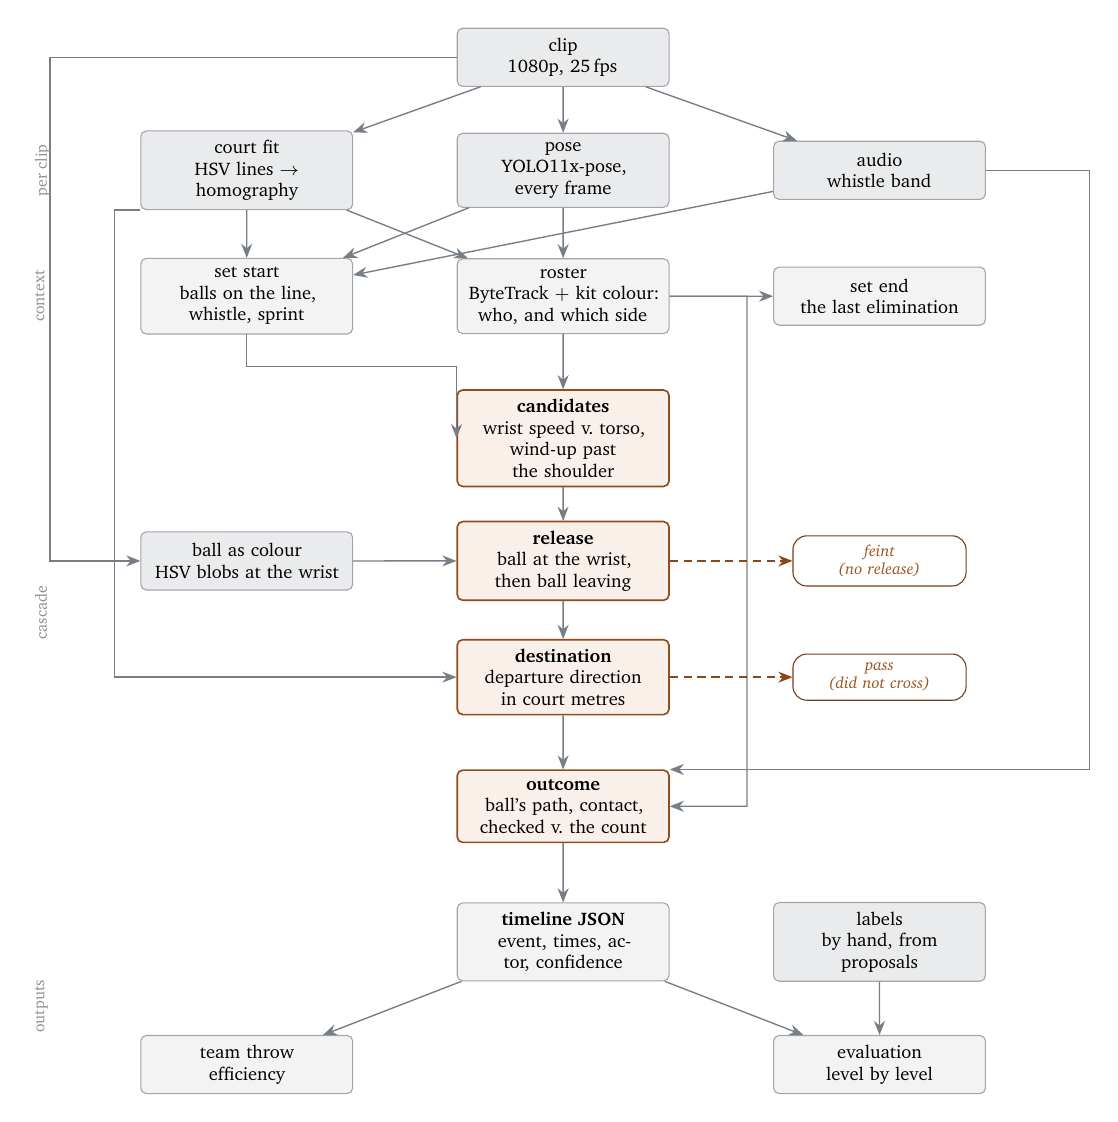
\begin{tikzpicture}[
  scale=0.82, every node/.style={transform shape},
  font=\small,
  stage/.style={draw=slate!55, fill=white, rounded corners=2pt, align=center,
                inner sep=4pt, minimum height=9mm, text width=30mm, font=\footnotesize},
  src/.style={stage, fill=slate!10, draw=slate!45},
  cas/.style={stage, draw=accent!75!black, fill=accent!10, line width=0.6pt},
  res/.style={stage, fill=slate!6, draw=slate!45},
  term/.style={draw=accent!60!black, fill=white, rounded corners=5pt, align=center,
               inner sep=4pt, text width=24mm, font=\scriptsize\itshape,
               text=accent!80!black},
  ar/.style={-{Stealth[length=1.8mm,width=1.4mm]}, draw=slate!65, line width=0.5pt},
  dar/.style={ar, densely dashed, draw=accent!70!black},
  lay/.style={font=\scriptsize, text=slate!55, anchor=west},
]

\node[src] (vid) at (0,0) {clip\\1080p, 25\,fps};

\node[src] (court) at (-4.9,-1.75) {court fit\\HSV lines $\to$ homography};
\node[src] (pose)  at (0,-1.75)    {pose\\YOLO11x-pose,\\every frame};
\node[src] (audio) at (4.9,-1.75)  {audio\\whistle band};

\node[res] (ss)    at (-4.9,-3.7) {set start\\balls on the line, whistle, sprint};
\node[res] (ros)   at (0,-3.7)    {roster\\ByteTrack $+$ kit colour:\\who, and which side};
\node[res] (se)    at (4.9,-3.7)  {set end\\the last elimination};

\node[cas] (cand) at (0,-5.9) {\textbf{candidates}\\wrist speed v.\ torso,\\wind-up past the shoulder};
\node[cas] (rel)  at (0,-7.8) {\textbf{release}\\ball at the wrist,\\then ball leaving};
\node[cas] (dest) at (0,-9.6) {\textbf{destination}\\departure direction\\in court metres};
\node[cas] (outc) at (0,-11.6) {\textbf{outcome}\\ball's path, contact,\\checked v.\ the count};

\node[src] (ball) at (-4.9,-7.8) {ball as colour\\HSV blobs at the wrist};

\node[res] (tl)   at (0,-13.7) {\textbf{timeline JSON}\\event, times, actor, confidence};
\node[res] (met)  at (-4.9,-15.6) {team throw\\efficiency};
\node[res] (ev)   at (4.9,-15.6) {evaluation\\level by level};
\node[src] (lab)  at (4.9,-13.7) {labels\\by hand, from proposals};

\node[term] (fake) at (4.9,-7.8) {feint\\(no release)};
\node[term] (pass) at (4.9,-9.6) {pass\\(did not cross)};

\draw[ar] (vid) -- (court);
\draw[ar] (vid) -- (pose);
\draw[ar] (vid) -- (audio);
\draw[ar] (vid.west) -- ++(-6.3,0) |- (ball.west);

\draw[ar] (pose)  -- (ss);
\draw[ar] (audio) -- (ss);
\draw[ar] (court) -- (ss);
\draw[ar] (pose)  -- (ros);
\draw[ar] (court) -- (ros);
\draw[ar] (ros)   -- (se);

\draw[ar] (ros) -- (cand);
\draw[ar] (ss.south) -- ++(0,-0.5) -| (cand.west);
\draw[ar] (cand) -- (rel);
\draw[ar] (ball) -- (rel);
\draw[ar] (rel)  -- (dest);
\draw[ar] (dest) -- (outc);
\draw[ar] (court.south west) -- ++(-0.4,0) |- (dest.west);
\draw[ar] (ros.east) -- ++(1.2,0) -- ++(0,-7.9) -- (outc.east);
\draw[ar] (audio.east) -- ++(1.6,0) |- (outc.north east);

\draw[dar] (rel.east)  -- (fake.west);
\draw[dar] (dest.east) -- (pass.west);

\draw[ar] (outc) -- (tl);
\draw[ar] (tl)  -- (met);
\draw[ar] (tl)  -- (ev);
\draw[ar] (lab) -- (ev);

\node[lay] at (-8.3,-1.75) {\rotatebox{90}{\makebox[0pt]{per clip}}};
\node[lay] at (-8.3,-3.7)  {\rotatebox{90}{\makebox[0pt]{context}}};
\node[lay] at (-8.3,-8.6)  {\rotatebox{90}{\makebox[0pt]{cascade}}};
\node[lay] at (-8.3,-14.7) {\rotatebox{90}{\makebox[0pt]{outputs}}};

\end{tikzpicture}
\caption{Footage in, timeline and metric out, as designed. The four orange stages are the
cascade and the dashed exits are where a candidate stops being a throw. Each stage writes
one file and the next reads it.}
\label{fig:pipeline}
\end{figure}

\subsection{The stages}

{\footnotesize
\begin{xltabular}{\textwidth}{L{30mm} L{34mm} X}
\toprule
\textbf{Stage} & \textbf{Writes} & \textbf{What it decides}\\
\midrule
\texttt{fit\_court} & \texttt{data/court/} & Homography between image and court metres, the centre line, the margin band, and a scale model for normalising features by depth\\
\texttt{precompute\_pose} & \texttt{data/pose/} & Every person, every frame, once per clip. Shared by the pipeline and the labelling tool so both see the same detections\\
\texttt{detect\_set\_start} & \texttt{data/sets/} & Where each set begins: balls on the centre line arm a window, a whistle inside it is the start, the teams breaking for the balls confirms it\\
\texttt{identify\_players} & \texttt{data/roster/} & Who is a player and which side, from tracks and kit colour\\
\texttt{detect\_set\_end} & \texttt{data/sets/} & Where each set ends, the last elimination\\
\texttt{detect\_candidates} & \texttt{data/candidates/} & Throwing motions, proposed loose\\
\texttt{detect\_events} & \texttt{data/timeline/} & The cascade: released or not, pass or throw, and the outcome\\
\texttt{evaluate} & \texttt{output/} & Every level scored against the labels, plus the metric\\
\bottomrule
\end{xltabular}}

Each stage is its own script and writes its own file, so any stage can be rerun or
inspected on its own, and a degraded copy of the clip for the stress test is simply a new
clip with its own files. \texttt{scripts/run.py} runs the stages in
the only order that works and stops at the first failure.

\subsection{Two contracts every stage shares}

\begin{itemize}
\item \textbf{The clip hash.} Every derived file records the SHA-256 of the clip it was
computed from and every reader refuses a mismatch. Frame indices are the only thing tying
calibration, detections, labels and timeline together, and a re-encode shifts them without
changing a filename.
\item \textbf{The venue is a file.} What is assumed about \emph{this} venue and \emph{this}
footage, the ball's colour window, the court's dimensions, the kit colours, lives in one
config file and nowhere else. Algorithm tunings stay out of it, as named constants beside the
code that owns them. A second venue should be a config change plus a retune, not a rewrite.
\end{itemize}

%=====================================================================
\section{Signal strategy}
\label{sec:signals}

\subsection{The signals considered}

{\footnotesize
\begin{xltabular}{\textwidth}{L{31mm} L{34mm} X L{18mm}}
\toprule
\textbf{Signal} & \textbf{What it gives} & \textbf{Where it fails} & \textbf{Role}\\
\midrule
Pose sequence (wrist, elbow, shoulder over $\sim$0.5\,s) & Wind-up onset, throwing arm, the candidate itself & Far-court players at half the pixel height, occlusion by teammates, side-on arm ambiguity & \textbf{primary} for candidates\\
Pose at and after the peak (follow-through, arm extension, speed decay) & Possibly feint versus throw & Unknown. A feint is the same motion with the ball kept, so this may carry nothing & to test\\
Ball colour at the wrist & Was there a ball to release & Ball hidden between two bodies, a hue close to the kit & \textbf{primary} for release\\
Ball seen leaving & Release, and the first metre of flight & Motion blur, a second ball crossing the wrist & \textbf{primary} for release\\
Departure direction in court metres v.\ the centre line & Pass or throw & Shallow releases near the line, lobbed passes & \textbf{primary} for destination\\
Short post-release trajectory & Direction, target side, outcome & Crosses other balls, leaves frame & \textbf{primary} for outcome\\
On-court count per side & Hit, catch, and which side lost someone & Eliminations that are not throw outcomes, tracker dropouts & check on outcome\\
Court homography & Which side, the far boundary, depth normalisation & Pan or zoom, few visible markings & geometry layer\\
Audio, whistle band & Set start, and outcome corroboration & Crowd noise, commentary & set start; fusion ablation\\
Global multi-ball tracking & Ball possession counts & Six near-identical balls in constant hand-off & \textbf{rejected}\\
\bottomrule
\end{xltabular}}

\changed{Two of these did not hold. Pose at the peak does not separate a feint from a
throw, every feature tried sits near chance, so the ball alone decides release. The whistle
band fires far too often during play to mean anything without other signals, so audio is
used only at the set start, where the ball line-up gives it a window. Report \S3.}

\subsection{Primary approach}

Pose finds the motion: the feasibility check (\S\ref{sec:feas}) says the arm keypoints are
clean at near-court scale and coarse but present at far-court scale. The ball decides
release, because a feint is a throw with the ball kept and whatever separates them has to be
about the ball; follow-through and arm extension get tested because they are cheap, but the
design does not depend on them. Direction decides pass versus throw, because a pass leaves no
trace in game state and where the ball went is the only evidence; the court homography turns a
departure vector in pixels into a side of the centre line.

\changed{Direction is taken in the image, not in court metres, plus contact with a player's
box where the trajectory reaches one. The floor homography cannot place a ball in the air.
Report \S3.}

The trajectory decides outcome, checked against the count: the ball after release says
which side it went to and roughly where it ended, and what happened to the player it reached
says whether that was a hit, a catch or a miss.

\subsection{Why HSV and not a detector}

HSV is cheap, fast, and enough for what the event needs: the ball at the thrower's wrist
and along its first metre of flight, both of which colour gives at this camera. A learned
detector is the better long-term choice, but with six balls in play it would need
fine-tuning and reliable linking, and that is not worth the budget for a proof of concept.
The trigger for building one is the colour mask becoming the limit, a venue where the kit
shares the ball's hue or a resolution where the ball is a few pixels. The same reasoning
rules out global multi-ball tracking.

%=====================================================================
\section{Models and methods}

{\footnotesize
\begin{xltabular}{\textwidth}{L{29mm} L{30mm} X}
\toprule
\textbf{Job} & \textbf{Chosen} & \textbf{Trade-off, and what was rejected}\\
\midrule
Person detection $+$ keypoints & Ultralytics YOLO11x-pose,\footnote{G.\ Jocher, J.\ Qiu
and A.\ Chaurasia, \emph{Ultralytics YOLO} (version 8.4), software, 2024,
$<$\url{https://github.com/ultralytics/ultralytics}$>$, accessed 27 August 2026.}
1920\,px, every frame & The largest pose model at full input resolution, because far-court players are half the height of near ones and the arm keypoints are the whole signal. This is the pipeline's entire compute budget (\S\ref{sec:compute}). Smaller variants and 640\,px inference are the fallback if it is too slow, at the far court's expense\\
Tracking & ByteTrack,\footnote{Y.\ Zhang, P.\ Sun, Y.\ Jiang, D.\ Yu, F.\ Weng,
Z.\ Yuan, P.\ Luo, W.\ Liu and X.\ Wang, `ByteTrack: Multi-Object Tracking by
Associating Every Detection Box', in \emph{Computer Vision -- ECCV 2022}, Lecture Notes in
Computer Science 13682 (Cham: Springer, 2022), pp.\ 1--21.} via Ultralytics & Off the shelf and good enough over precomputed detections. Fragments are expected and are what kit colour and, if time allows, jersey numbers repair. Re-identification embeddings are not worth it for twelve players in two kits\\
Team and identity & Kit colour for team; EasyOCR\footnote{JaidedAI, \emph{EasyOCR}
(version 1.7), software, $<$\url{https://github.com/JaidedAI/EasyOCR}$>$, accessed
27 August 2026; its detector is Y.\ Baek, B.\ Lee, D.\ Han, S.\ Yun and H.\ Lee,
`Character Region Awareness for Text Detection', in \emph{2019 IEEE/CVF Conference on
Computer Vision and Pattern Recognition} (Long Beach, 2019), pp.\ 9357--9366.} on jersey
crops for player identity, budget permitting & Team is required for the metric and kit colour is reliable at this camera. Player identity is reported where a track is stable and a number is readable\\
Court geometry & Median background plate, HSV line extraction, homography to metres, with a held-out check on markings not used in the fit & A known method, and quicker to run than hand-labelling the corners would have been; the venue is ideal for it, one fixed camera and clean markings on a plain floor. It also gives metres, a scale model and a drift check that a hand-drawn polygon would not. Rejected: inference on rectified imagery, since a floor homography stretches upright bodies into shapes no pose model has seen\\
Ball & HSV blob detector, ball-sized components, hue floor set above the red kit & \S\ref{sec:signals}. Cheap, and it holds at 20\,px where a stock detector drops out on blur. Cannot see a ball against the red team at the far baseline\\
Wind-up & Wrist speed relative to torso, normalised by depth, peak-picking with a score floor & Loose, because a missed candidate is unrecoverable and a rejection costs one keypress in the labelling tool. A learned temporal model is rejected on data volume, sixty events is not a training set\\
Temporal logic & Explicit gates and named constants & Every decision is a threshold on a measured quantity with the reason for its value beside it. Rejected: a fused score, which blends four independent failure modes into one number\\
\bottomrule
\end{xltabular}}

\textbf{Nothing is trained.} Every component is pretrained or analytic. With a few dozen
labelled events any learned event model would be fitting the evaluation set. Where training
would first pay is in \S\ref{sec:failure}.

%=====================================================================
\section{Data and labels}

\subsection{Footage}

Two sources were compared.

{\footnotesize
\begin{xltabular}{\textwidth}{L{22mm} X X}
\toprule
 & \textbf{WDBF 2014 men's final, Canada v.\ USA, 2nd half}\footnote{World Dodgeball
Federation, \emph{2014 World Dodgeball Championship, Men's Final: Canada v USA} [video],
YouTube, $<$\url{https://www.youtube.com/watch?v=Spu6OlAZHUo}$>$, accessed 27 August 2026.}
& \textbf{Sky Zone Ultimate Dodgeball 2014}\\
\midrule
Camera & One fixed elevated end-on camera for the whole half & Produced broadcast: cuts every few seconds, replays, commentators\\
Format & 25\,fps, 1920$\times$1080 & 30\,fps, 1920$\times$1080\\
Game & WDBF foam, 6-a-side, court fully in frame & Trampoline dodgeball, players airborne much of the time\\
Verdict & \textbf{primary} & Rejected. Cuts, re-identification across shots and replay de-duplication would swallow the budget, and ``three minutes continuous'' is murky when continuity is cut every few seconds\\
\bottomrule
\end{xltabular}}

The evaluation clip is 6:00 to 9:30 of the half: one complete set from the opening rush to
the next, 3.5 minutes. All twelve players start on court, so the throw rate is at its
highest. It has about 18 seconds of pre-set at the start and a partial lens obstruction part-way
through. The following set is the held-out segment.

Footage is never committed, for licensing and size. Two scripts obtain it and cut the clip,
re-encoding so that frame indices are exact.

\subsection{Feasibility check}
\label{sec:feas}

Ten seconds of the clip were run through the intended pose model before the design was
fixed.

{\footnotesize
\begin{xltabular}{\textwidth}{L{44mm} L{28mm} X}
\toprule
\textbf{Observation} & \textbf{Measured} & \textbf{Consequence}\\
\midrule
People per frame & 38.5 mean, against 12 on court & Sidelines, bench, referees and crowd. The court polygon filters them, and the fixed camera means no per-frame work\\
Near-team box height & 280\,px median & Full skeletons, clean arm keypoints, wind-ups clearly resolvable\\
Far-team box height & 150\,px median, 91\,px at p10 & Skeletons present, arm keypoints coarse. Far-court detection will be weaker and is reported separately\\
Ball in hand, near court & 40--50\,px, orange on red and grey & Unmistakable unless between two bodies\\
Ball in flight, far court & 15--20\,px, still an obvious orange blob & Colour carries a lot. An HSV detector is viable\\
\bottomrule
\end{xltabular}}

\subsection{Labels}
\label{sub:labels}

\textbf{Ground truth.} No public dodgeball event dataset exists, so it is labelled here. The target is
at least twenty events; the estimate for one set is 50 to 70 throws plus 10 to 20 feints at
about 45 seconds each, around an hour with a purpose-built tool. How often teams pass is
unmeasured, and it sets both the labelling cost and how much the denominator depends on pass
rejection.

\textbf{The labelling tool.} We will build our own labeller, since the right tool makes
the work quicker and less error prone. It will show the pose run over the video with a key
for each player on the field, so the thrower and target attach to an event in one press,
and every action is a keybinding. It will be bootstrapped with a simple wrist-speed model
tuned for recall over precision; I then review each proposal and correct the labels,
scrubbing the clip for anything the proposer missed. The cost of bootstrapping is that
candidate recall is measured against a truth set the candidate stage seeded, so it reads as
the precision of a recall-tuned stage.

\textbf{Anchor on the release frame.} It is the crispest moment and the one the temporal
tolerance is measured against.

\textbf{Player boxes.} A player is stored as a box in source pixels on the
frame it was placed, the thrower at release and the target at the end. Evaluation matches
boxes to any detector's output, so nothing the detector does later can change what a label
means.

\textbf{Separating label uncertainty from model error.} Each event records
\texttt{release\_visible}, \texttt{outcome\_visible}, \texttt{ref\_signal} (the closest
thing to external truth on a contested hit), an \texttt{uncertain} flag and a note. These
are the error budget's label term.

\textbf{Double-label a subset.} About twenty events, second pass done blind, to measure
agreement on the release frame and the outcome. This is the label-uncertainty term in the
error budget.

\textbf{Not labelled.} Non-throw negatives (hand-offs, pickups, retrieval rolls); every
false positive gets a cause category during analysis instead. Eliminations follow from
outcome and target.

\subsection{The annotation rule handed to another person}

\texttt{docs/labeling-guide.md}, written to stand without this document. It fixes the
release-frame anchor, where thrower and target are clicked, team from the court half,
\texttt{kind} by destination, what is not a candidate, and the four ambiguous cases
(occluded release, graze versus dodge, crossing balls, unobserved destination) with the flag
to set and the fallback to use for each.

%=====================================================================
\section{Evaluation}
\label{sec:eval}

\subsection{One score per level}

Matching is same-frame, same-player: a prediction matches a labelled event when the release
frames are within tolerance \emph{and} the thrower boxes overlap.

{\footnotesize
\begin{xltabular}{\textwidth}{L{26mm} L{40mm} X}
\toprule
\textbf{Level} & \textbf{Metric and tolerance} & \textbf{What the number misses}\\
\midrule
Candidate & Precision / recall / F1 at $\pm$0.25\,s ($\pm$6 frames at 25\,fps) and IoU $\geq$ 0.5 on the thrower & Recall is against a truth set this stage seeded (\S\ref{sub:labels}). Precision is scored against unlabelled negatives, so a wound-up ball the annotator did not call a feint counts against it\\
Boundaries & Mean absolute error on \texttt{start} and \texttt{end} for matched events & Softer moments than release; expect wide error\\
Attribution & Team accuracy; player accuracy where the track is stable & Team is nearly free at this camera. Player-level attribution only means anything for players whose identity is stable\\
Kind & Feint / pass / throw accuracy on matched events, feints reported separately & With few labelled passes the pass column has a wide interval\\
Outcome & Accuracy and a confusion matrix over the five classes, on matched throws & Small denominator, and \texttt{unresolved} has to be kept apart from wrong\\
Metric & Absolute error in throw efficiency per team & Numerator and denominator errors can cancel. The error budget exists to catch that\\
\bottomrule
\end{xltabular}}

The $\pm$0.25\,s tolerance is about the window a second annotator would place a release
in.

\subsection{Stress}

Three conditions, each chosen to break a different thing, with tolerance unchanged. Every
pixel-reading stage is rerun on the degraded clip; the court fit, set boundaries and labels
are carried over as deterministic transforms of the source, so what is measured is the
vision.

{\footnotesize
\begin{xltabular}{\textwidth}{L{22mm} L{38mm} X}
\toprule
\textbf{Condition} & \textbf{What it degrades} & \textbf{What we expect it to break}\\
\midrule
480p downscale & Spatial resolution & The ball (8\,px is a few pixels of hue) and far-court keypoints\\
Heavy compression (high CRF) & Blocking artefacts & Pose itself, and therefore the wind-up detector's precision\\
Frame dropping (every second frame) & Temporal resolution & The release check, which needs consecutive frames of the ball leaving\\
\bottomrule
\end{xltabular}}

\subsection{Ablation}

One pipeline run scored three times with the later stages withheld: pose only (every
proposal is a throw, the simple baseline), plus the release gate (released means throw),
plus destination (pass or throw). The candidate matching is identical in every row; what
moves is what each stage claims about the same motion. This prices the two structured
negatives separately, which matters because they cost the metric differently. A fusion
ablation, vision only against vision plus whistle, is the second comparison if audio earns
its place.

\subsection{Error budget}

Three terms. \textbf{Model}: a paired bootstrap over
matched events, giving a 95\% band on predicted minus truth efficiency per team.
\textbf{Labels}: efficiency recomputed with every \texttt{uncertain} event decided the other
way, plus the double-label agreement. \textbf{Sampling}: a Wilson interval on the truth
itself. With fifteen throws a side the sampling term will probably dominate, in which case
one set cannot measure a team, which is the argument for the pipeline.

%=====================================================================
\section{Compute and latency}
\label{sec:compute}

\textbf{Batch.} Pose is essentially the whole cost and everything after it
should be seconds.

{\footnotesize
\begin{xltabular}{\textwidth}{L{34mm} L{30mm} X}
\toprule
\textbf{Stage} & \textbf{Budget, 3.5\,min clip} & \textbf{Basis}\\
\midrule
Pose (YOLO11x-pose, 1920\,px, half precision) & $\sim$5\,min & About 18\,fps on a laptop RTX 4080, measured on ten seconds of the clip. Chunked and resumable, since it is the one stage not cheap to rerun\\
Court fit & Seconds, once per clip & A median plate and a line fit\\
Tracking $+$ identity & Under a minute & Tracking over precomputed detections; OCR on selected crops only\\
Candidates, release, destination, outcome & Seconds to a minute & Arithmetic over the pose run, plus one sequential decode of the clip around each proposal for the ball\\
Evaluation, error budget & Seconds & \\
\midrule
\textbf{Training} & \textbf{none} & Every component is pretrained or analytic\\
\bottomrule
\end{xltabular}}

\textbf{Latency.} As designed the system is batch: a clip in, a timeline out. Near real
time is reachable, because nothing in the cascade needs the future beyond a fixed short
window: the trajectory is followed a few hundred milliseconds past release, and the count
check holds for a second or two. So the floor is a few seconds behind live, per event.
Frame-level real time is not reachable and not needed for a metric reported per set.

\textbf{Throughput.} Pose is the bottleneck at about 18\,fps against 25\,fps of footage.
Two ways to close the gap, in the order we would try them:
\begin{itemize}
\item \emph{Parallelise.} Pose is per frame with no state between frames, so the clip splits
into chunks that run on separate GPUs (AWS Batch or similar) and wall-clock falls with the
number of workers. No accuracy cost.
\item \emph{Speed up one GPU.} TensorRT export first; a smaller pose variant or a lower
input resolution last, since both cost accuracy at the far court, which is what full
resolution is buying. Half precision is already assumed above: it doubles throughput at this
model size for a sub-pixel change in keypoints. Batching does not help, one 1920\,px frame
already fills the GPU.
\end{itemize}

%=====================================================================
\section{Failure modes}
\label{sec:failure}

Where we expect the system to break first, and how we would find out.

{\footnotesize
\begin{xltabular}{\textwidth}{L{30mm} L{62mm} X}
\toprule
\textbf{Failure} & \textbf{Why} & \textbf{How to test or reduce it}\\
\midrule
Feints read as throws & Pose alone cannot tell them apart and the ball check depends on seeing the ball at the wrist & The ablation prices it directly. If the release gate does not buy precision, the ball detector is the next model\\
Passes read as throws & Shallow releases near the centre line, lobbed passes; and no game-state check exists for a pass & Report the pass column on its own. More labelled passes are the only real fix, and the clip may not have many\\
Far-court recall & Half the pixel height, coarse arm keypoints & Report near and far separately. Reducing it means resolution, which means compute\\
Outcome attributed to the wrong throw & Coordinated attacks put several releases within 200\,ms and balls cross in flight & Attribute by thrower, never by following the ball. The count check catches an impossible sequence but cannot say which of two throws did it\\
Occluded release & The thrower's hand hidden by a teammate at the moment that matters & Unobservable. Label it as such (\texttt{release\_visible}) so it lands in the label term, not the model term\\
The ball is a colour & The mask cannot see the ball against a same-hue kit or at a few pixels & The 480p stress condition measures it. That is the trigger for a learned detector\\
Identity & Tracker swaps in pile-ups; unreadable numbers on one kit & Attribute by team, which is what the metric needs. Player-level claims only where a number is read\\
A second venue & Court fit, ball colour and kit colours are all this footage's & Fail loudly: the court fit checks itself against held-out markings, the venue file refuses unknown keys, every derived file refuses a clip it was not computed from\\
\bottomrule
\end{xltabular}}

The biggest structural risk is the outcome. Every other failure degrades gracefully; an
outcome on the wrong throw is two errors at once, one invented and one missed, both in the
metric's numerator.

%=====================================================================
\section{What changed in the build}
\label{sec:changed}

Three decisions above are marked
\textcolor{accent!88!black}{$\triangleright$}. The outcome is read from the on-court count
rather than the ball's trajectory. Audio is used at the set start only. Pass versus throw is
decided by the ball's direction in the image and by contact with a player, not by direction
in court metres. Two things were planned and not done: the per-event confidence, and the
blind second labelling pass. Each of these has its measurement and its reasoning in the report,
and the shipped design of each stage is in \texttt{docs/architecture/}.

%=====================================================================
\section*{Bibliography}
\addcontentsline{toc}{section}{Bibliography}

\raggedright\sloppy
\begin{itemize}[leftmargin=1.4em,label={},itemsep=4pt]
\item Baek, Y., Lee, B., Han, D., Yun, S. and Lee, H., `Character Region Awareness for
Text Detection', in \emph{2019 IEEE/CVF Conference on Computer Vision and Pattern
Recognition} (Long Beach, 2019), pp.\ 9357--9366.
\item Hu, A., `Leveraging AI Video Frame Recognition to Quantify Ball Possession',
\emph{Medium}, December 2025,
$<$\url{https://medium.com/@arthurwang0815/leveraging-ai-image-recognition-to-quantify-ball-possession-e6493d8428e1}$>$,
accessed 27 August 2026.
\item JaidedAI, \emph{EasyOCR} (version 1.7), software,
$<$\url{https://github.com/JaidedAI/EasyOCR}$>$, accessed 27 August 2026.
\item Jocher, G., Qiu, J. and Chaurasia, A., \emph{Ultralytics YOLO} (version 8.4),
software, 2024, $<$\url{https://github.com/ultralytics/ultralytics}$>$, accessed
27 August 2026.
\item Nojima, T., Phuong, N., Kai, T., Sato, T. and Koike, H., `Augmented dodgeball', in
\emph{Proceedings of the 6th Augmented Human International Conference} (AH~'15),
Singapore, 2015, pp.\ 137--140.
\item World Dodgeball Federation, \emph{WDBF Dodgeball Rules 2024} (2024),
$<$\url{https://worlddodgeballfederation.com/wdbf-content/uploads/2024/03/WDBF-Dodgeball-Rules-2024.pdf}$>$,
accessed 27 August 2026.
\item World Dodgeball Federation, \emph{2014 World Dodgeball Championship, Men's Final:
Canada v USA} [video], YouTube, $<$\url{https://www.youtube.com/watch?v=Spu6OlAZHUo}$>$,
accessed 27 August 2026.
\item Zhang, Y., Sun, P., Jiang, Y., Yu, D., Weng, F., Yuan, Z., Luo, P., Liu, W. and
Wang, X., `ByteTrack: Multi-Object Tracking by Associating Every Detection Box', in
\emph{Computer Vision -- ECCV 2022}, Lecture Notes in Computer Science 13682 (Cham:
Springer, 2022), pp.\ 1--21.
\end{itemize}

\vspace{4mm}
\noindent{\small\color{mute}\rule{\textwidth}{0.4pt}\\[3pt]
Claude Code was used throughout: drafting modules and tests against a design agreed first,
running the evaluations, and writing the architecture documentation as each stage shipped.
Every label was placed by hand.}

\end{document}
